\chapter{Kravspecifikation}

\section{Use Case diagram}

\begin{figure}[h]
\centering
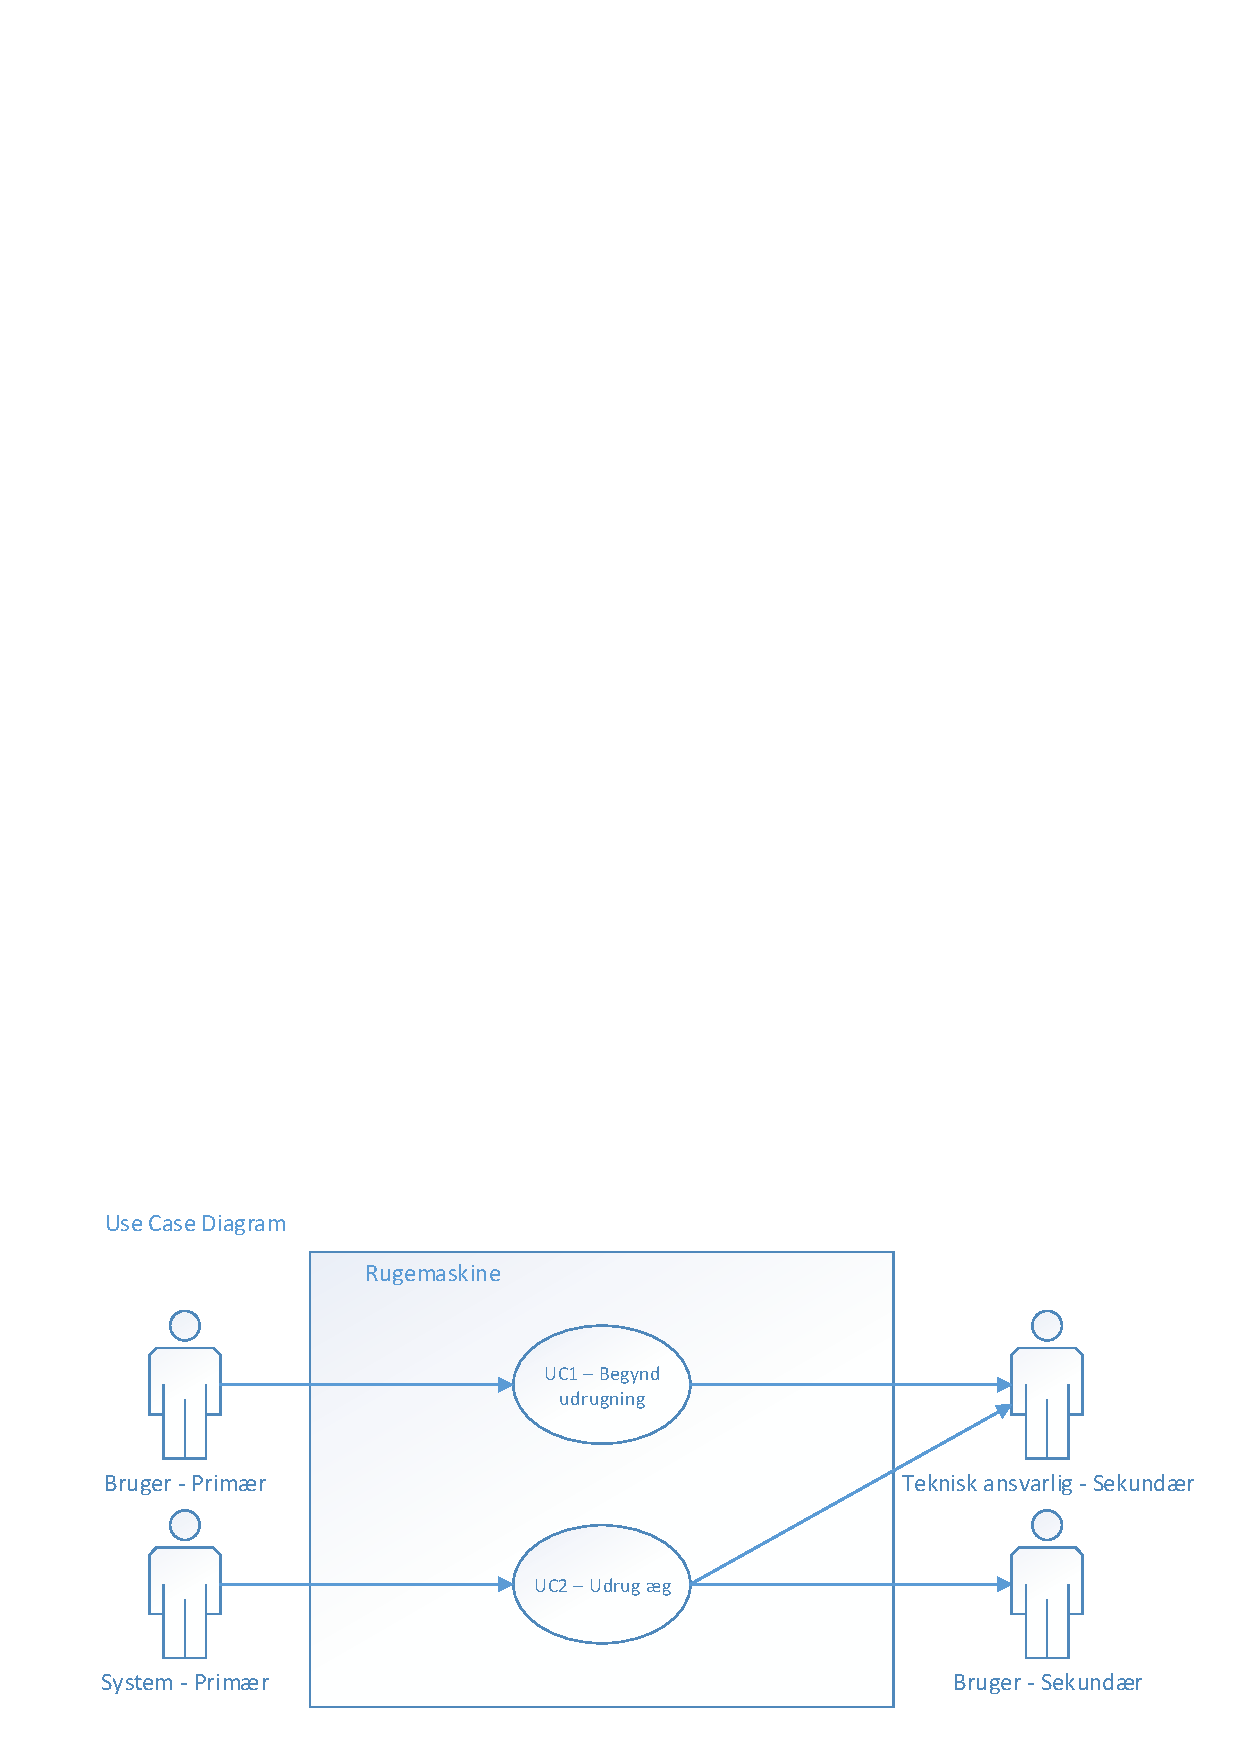
\includegraphics[width=16cm, scale=1, trim= 0mm 0mm 0mm 200mm, clip=true,  angle=0]{1_kravspecifikation/diagrammer/UseCase_Generel_v1.pdf}
\caption{Use Case diagram}
\label{fig:usecase_diagram}
\end{figure}

\clearpage
\section{Aktørbeskrivelse}

\subsection{Bruger}

\begin{table}[H]
\centering
\begin{tabular}[\textwidth]{|p{0.20\textwidth}|p{0.80\textwidth}|}
\hline Aktørnavn: & Bruger \\ 
\hline Alternativt navn: & User \\ 
\hline Type: & Primær og sekundær\\ 
\hline Beskrivelse: & 
		\begin{enumerate}
		\item Bruger ønsker at udruge æg
		\end{enumerate} \\ 
\hline
\end{tabular}
\caption{Aktør - Bruger}
\label{tab:usecase-aktoer-bruger}
\end{table}



\subsection{System}

\begin{table}[H]
\centering
\begin{tabular}[\textwidth]{|p{0.20\textwidth}|p{0.80\textwidth}|}
\hline Aktørnavn: & System \\ 
\hline Alternativt navn: & Rugemaskine \\ 
\hline Type: & Primær \\ 
\hline Beskrivelse: & 
		\begin{enumerate}
		\item Systemet styrer udrugningsprocesser.
		\item Systemet har til opgave at overvåge temperatur, luftfugtighed samt tidsprogression.
		\end{enumerate} \\ 
\hline
\end{tabular}
\caption{Aktør - System}
\label{tab:usecase-aktoer-system}
\end{table}



\subsection{Tekniske ansvarlig}

\begin{table}[H]
\centering
\begin{tabular}[\textwidth]{|p{0.20\textwidth}|p{0.80\textwidth}|}
\hline Aktørnavn: & Tekniske ansvarlig \\ 
\hline Alternativt navn: & Servicetekniker \\ 
\hline Type: & Ekstern \\ 
\hline Beskrivelse: & 
		\begin{enumerate}
		\item Tekniske ansvarlig er en uddannet tekniker, der har en faglig forståelse for opbygning af rugemaskinen.
		\end{enumerate} \\ 
\hline
\end{tabular}
\caption{Aktør - Tekniske ansvarlig}
\label{tab:usecase-aktoer-tekniskeansvarlig}
\end{table}


\clearpage

\section{Use Cases}
\subsection{Begynd udrugning}

\begin{table}[H]
\centering
\begin{tabular}[\textwidth]{|p{0.18\textwidth}|p{0.82\textwidth}|}
\hline Navn & Begynd udrugning \\ 
\hline Usecase ID & \usecaseset{Begynd udrugning} \\ 
\hline Scope &  \\
\hline Primær aktør & Bruger \\ 
\hline Interessenter & Tekniske ansvarlig. \\ 
\hline Forudsætning & Use Case \usecaseref{Udrug aeg} er ikke aktiv \\ 
\hline Resultat & Udrugning af indlagte æg er påbegyndt. \\ 
\hline Hovedforløb &
	\begin{enumerate}
	\item \label{itm:Begynd-step1} Bruger åbner låge.
	\item \label{itm:Begynd-step2} Systemet registrerer åbning af låge. 
	\item \label{itm:Begynd-step3} Systemet låser for interfacet (skriver "låge åben").
	\item \label{itm:Begynd-step4} Bruger placerer æg i maskine.
	\item \label{itm:Begynd-step5} Bruger lukker låge.
	\item \label{itm:Begynd-step6} Systemet registrerer lukning af låge.  
	\item \label{itm:Begynd-step7} Systemet låser op for interfacet (fjerner "låge åben").
	\item \label{itm:Begynd-step8} Bruger vælger type af æg til udrugning (sekvens).
	\item \label{itm:Begynd-step9} Systemet spørger bruger om bekræftelse.
	\item \label{itm:Begynd-step10} Bruger bekræfter valg (vælger "OK").
	\item \label{itm:Begynd-step11} Systemet registrerer valg.
	\item \label{itm:Begynd-step12} Systemet aktiverer sekvensen Udrug Æg (Use Case \usecaseref{Udrug aeg}).
%	\item \label{itm:Begynd-step12} 
	\end{enumerate} \\
	\hline Undtagelser &
	\begin{enumerate}
	\item[\ref{itm:Begynd-step2}a.] System registrerer ikke åbning af låge. 
	\begin{itemize}
	\item Bruger kontakter teknisk ansvarlig. 
	\end{itemize}
	\item[\ref{itm:Begynd-step6}a.] System registrerer ikke lukning af låge.  
	\begin{itemize}
	\item Bruger kontakter teknisk ansvarlig. 
	\end{itemize}
	\item[\ref{itm:Begynd-step10}a.] Bruger bekræfter ikke valg (vælger "Annullér"). 
	\begin{itemize}
	\item Step \ref{itm:Begynd-step8} gentages.
	\end{itemize}
	\end{enumerate} \\
\hline 
\end{tabular}
\caption{Use Case - Begynd udrugning}
\label{tab:usecase-Begynd-udrugning}
\end{table}
\linespread{1.0}\subsection{Udrug {\ae}g}
\begin{table}[H]
\centering
\begin{tabular}[\textwidth]{|p{0.18\textwidth}|p{0.82\textwidth}|}
\hline Navn & Udrug æg \\ 
\hline Usecase ID & \usecaseset{Udrug aeg} \\ 
\hline Primær aktør & System \\ 
\hline Interessenter & Sekundær aktør: Bruger \\ 
\hline Forudsætning & Use Case \usecaseref{Begynd udrugning} \\ 
\hline Resultat & Æggene er udruget og fjernet fra maskinen \\ 
\hline Hovedforløb &
	\begin{enumerate}
	\item \label{itm:udrugning-step1} Systemet indlæser valgte sekvens.
	\item \label{itm:udrugning-step2} Systemet regulerer temperatur og luftfugtighed.
	\item \label{itm:udrugning-step3} Systemet kontrollerer om det er tid til æggevending.  \newline
	\textbf{hvis} (tid = æggevending): Vend æg.
	\newline
	\textbf{ellers}: Vend ikke æg.
	\newline
	Step \ref{itm:udrugning-step2}-\ref{itm:udrugning-step3} gentages indtil udrugningstiden er afsluttet.
	\item \label{itm:udrugning-step4} 	System informerer brugeren om at udrugningssekvens er færdig.
	\item \label{itm:udrugning-step5} 	Bruger åbner låge.
	\item \label{itm:udrugning-step6} 	Systemet registrerer åbning af låge.
	\item \label{itm:udrugning-step7} 	Systemet afbryder regulering af temperatur og luftfugtighed.
	\item \label{itm:udrugning-step8} 	Bruger fjerner emne(r).
	\item \label{itm:udrugning-step9} 	Bruger lukker låge.
	\item \label{itm:udrugning-step10} 	Systemet registrerer lukning af låge.
	\item \label{itm:udrugning-step11} 	Systemet genoptager regulering af temperatur og luftfugtighed.
	\newline Step \ref{itm:udrugning-step5}-\ref{itm:udrugning-step11} gentages indtil brugeren indikerer overfor systemet at alle emner er fjernet.
	\item \label{itm:udrugning-step12}		Systemet stopper med regulering af temperatur og luftfugtighed.	
	\end{enumerate} \\
\hline Undtagelser &


\begin{enumerate}
		\item[*] Bruger afbryder udrugningen.
		\begin{itemize}
			\item Systemet afbryder Use Case \usecaseref{Udrug aeg}
		\end{itemize}
	\end{enumerate}

	\begin{enumerate}
		\item[*](\ref{itm:udrugning-step2}-\ref{itm:udrugning-step3}) Bruger åbner maskinen.
		\begin{itemize}
			\item Systemet afbryder trin 2-3.
			\begin{itemize}
				\item Bruger lukker maskinen.
				\item Systemet fortsætter med trin 2-3.
			\end{itemize}
		\end{itemize}
	\end{enumerate}

	\begin{enumerate}
	\item[\ref{itm:udrugning-step2}a.] Systemet kan ikke regulere temperatur eller luftfugtighed.
	\begin{itemize}
	\item Systemet registrerer fejl.
	\item Systemet informerer bruger om fejl.
	\end{itemize}
	\end{enumerate} 
	
	
	\begin{enumerate}
	\item[\ref{itm:udrugning-step6}a.]  System registrerer ikke åbning af maskine.
	\begin{itemize}
	\item Bruger kontakter tekniske ansvarlig.
	\end{itemize}
	\end{enumerate}  
	
	\begin{enumerate}
	\item[\ref{itm:udrugning-step10}a.]  System registrerer ikke lukning af maskine.
	\begin{itemize}
	\item Bruger kontakter tekniske ansvarlig.
	\end{itemize}
	\end{enumerate} \\ \hline 
\end{tabular}
\caption{Use Case - Udrug æg}
\label{tab:usecase-Udrug-aeg}
\end{table}
\clearpage

\section{Funktionelle krav}

\begin{enumerate}
 \item Systemet skal kunne regulere temperaturen efter justering af parameter inden for 10 min. 
 \item Systemet skal kunne regulere luftfugtigheden efter justering af parameter inden for 10 min.
\end{enumerate}
\FloatBarrier

\section{Ikke-funktionelle krav}

\begin{enumerate}

\item Hvis systemet ikke kan overholde de angivne grænser som er beskrevet i de funktionelle krav, skal brugeren informeres vha. alarmer.

\item DevKit8000 8000 anvendes som styrende enhed samt grafisk brugergrænseflade (GUI).

\item PSoC3 og/eller 4 anvendes som grænseflade til føler/sensorer samt aktuatorer.

\item Tilladte afvigelser:
	\begin{itemize}
	\item Temperatur: $\pm$ 1$^\circ$C.
	\item Luftfugtighed : $\pm$ 10 procentpoint.
	\end{itemize}

\item Krav til opstillingsmiljø:
	\begin{itemize}
	\item Temperatur : 15-30$^\circ$C.
	\item Luftfugtighed : <45\% procentpoint.
	\end{itemize}

\item krav til GUI:
	\begin{itemize}
	\item Der skal være mulighed for at navigere via GUI.
	\item GUI skal kunne bruges til at starte og stoppe udrugningen.
	\item Der skal altid på UI under udrugning fremgå: Temperatur, luftfugtighed, tidsprogression.
	\item GUI skal gøre bruger opmærksom på tilstandsændringer.
	\end{itemize}

\item Rugemaskinens dimensioner er: $\pm$ 2 cm
	\begin{itemize}
	\item Brede x cm
	\item Højde x cm
	\item Dybte x cm
	\end{itemize}
		
\item Udrugningsprocedurer skal følge anbefalingerne angivet på www.hønsehus.dk/opdraet/rugetips/

\item Rotation: Rotation på 180$^\circ$ $\pm$ 45$^\circ$

\end{enumerate}
\clearpage

%\section{Accepttestspecifikation}
%Da vi ikke formåede at sammensætte og teste systemet i dets helhed, kan vi ikke godkende nedenstående accepttests. Vi har dog gennemført og godkendt flere af testene i et "subset" af systemet, som inkluderede sammensatte moduler.

\subsection{Accepttestspecfikation for Use Case \usecaseref{Begynd udrugning}} 

%************************ Use Case 1 **************************************
 
 \subsubsection{Hovedscenarie}
\begin{center}

	\begin{tabular}{| p{3cm} | p{3cm} | p{3cm} | p{3cm} |}
		\hline
		Krav & Udførelse & Forventet resultat & Resultat \\ \hline
		% % % % % % % % % % % % % % % % % % % % % % % % % % % % 
		
		\multirow{2}{3cm}{Ved lågens åbning låses UI. Det forbliver låst indtil lågen lukkes.} 
		& Maskinen står i idle tilstand og lågen åbnes
		& UI låser
		& \\ \cline{2-4}
		
		&Lågen lukkes igen
		
		&UI låser op
		& \\ \hline 
		

	\end{tabular}
\end{center}

%\subsubsection{Undtagelser}
%\begin{center} 
%	\begin{tabular}{| p{3cm} | p{3cm} | p{3cm} | p{3cm} |}
%	\end{tabular}
%\end{center}

\subsection{Accepttestspecfikation for Use Case \usecaseref{Udrug aeg}} 

%************************ Use Case 2 **************************************
 
 \subsubsection{Hovedscenarie}
\begin{center}

	\begin{longtable}{| p{3cm} | p{3cm} | p{3cm} | p{3cm} |}
		\hline
		Krav & Udførelse & Forventet resultat & Resultat \\ \hline
		% % % % % % % % % % % % % % % % % % % % % % % % % % % % 
		
		
		Systemet skal kunne regulere og holde en temperatur indenfor grænserne angivet i ikke funktionelle krav.
		&Systemet opstilles i omgivelser der ligger indenfor de påkrævede rammer. Systemet indstilles til at skulle holde 37$^\circ$C. Systemet sættes i gang og temperaturen aflæses efter 10 minutter. 
		&Maskinen kan regulere og holde temperaturen indenfor de angivne rammer. 
		& \\ \hline
		
		Systemet skal kunne regulere og holde en luftfugtighed indenfor grænserne angivet i ikke funktionelle krav.
		&Systemet opstilles i omgivelser der ligger indenfor de påkrævede rammer. Systemet indstilles til at skulle holde 70\% relativ luftfugtighed. Systemet sættes i gang og luftfugtigheden aflæses efter 10 minutter.
		&Maskinen kan regulere og holde luftfugtigheden indenfor de angivne rammer.
		& \\ \hline
		
		Maskinen kan vende æg med et bestemt interval. Æggene roteres indenfor de i ikke funktionelle krav specificerede grænser.
		&Æg-type specificeres, og systemet indstilles til at skulle vende æggene hvert 5. minut i en periode på 30 minutter. Æggenes vertikale akse markeres med en pil, der peger op. Systemet sættes i gang og kører i 30 minutter. Ved hver vending måles rotation af hvert æg, og deres rotation noteres. Efter hver rotation vendes hvert æg manuelt så orienteringsindikatoren (pilen) peger opad. 
		&Maskinen roterer alle æg indenfor den angivne grænse.
		& \\ \hline		
		
		Systemet skal ved afsluttet udrugning informere brugeren om dette.
		&Maskine indstilles til et 5 minutters udrugningsprogram og igangsættes. Det observeres at systemet informerer brugeren når sekvensen afsluttes.
		&Maskinen vil ved testsekvensens afslutning informere brugeren.
		& \\ \hline

		
		
	\end{longtable}
\end{center}
\clearpage
\subsubsection{Undtagelser}
\begin{center}

	\begin{longtable}{| p{3cm} | p{3cm} | p{3cm} | p{3cm} |}
	\hline
			Krav & Handling & Forventet resultat & Resultat \\ \hline
			% % % % % % % % % % % % % % % % % % % % % % % % % % % % 
			
			\multirow{2}{\linewidth}{Ved lågens åbning låses UI og udrugningssekvensens afbrydes midlertidigt. UI forbliver låst indtil lågen lukkes. Når lågen lukkes genoptages udrugnings- sekvensen.} 
			& Maskinen står I udrug-tilstand og lågen åbnes. \newline
			& UI låser og udrugningssekvensen stoppes.
			& \vspace{2.5cm} \\ \cline{2-4}
			
			&Lågen lukkes igen.
			
			&UI låser op og udrygningssekvensen genoptages.
			& \vspace{2.5cm} \\ \hline 
			
			Hvis det ikke er muligt at overholde temperaturen skal systemet informere brugeren.
			&Maskine opstilles i et lokale med temperatur indenfor de angivne grænser for opstilningsmiljø. Systemet indstilles til at skulle holde temperaturen på 40$^\circ$C, varmelegemet frakobles, og systemet aktiveres. \newline
			&Maskinen informerer brugeren. 
			& \\ \hline
			
			Hvis det ikke er muligt at overholde luftfugtigheden skal systemet informere brugeren.
			
			&Maskine opstilles i et lokale med luftfugtighed indenfor de angivne grænser for opstilningsmiljø. Systemet indstilles til at skulle holde luftfugtigheden på 70\% relativ luftfugtighed, luftfugtighedsreguleringsmekanismen  frakobles, og systemet aktiveres.
			
			&Maskinen informerer brugeren.
			
			& \\ \hline
					
			
		\end{longtable}
	\end{center}